\chapter{PRINCIPAIS PROCESSOS DE VISÃO COMPUTACIONAL}

Este Capítulo contextualiza os principais processos da área de Visão Computacional. São descritas as técnicas mais utilizadas em cada um desses processos visando atingir o entendimento necessário para esse trabalho.

\section{Processamento de Imagem}

Processamento de Imagem é um processo da Visão Computacional que atua na maior parte dos projetos do universo bidimensional. Esse processo consiste em tratar a imagem buscando obter o máximo de qualidade possível sem se importar com a informação em si. Segundo \citeonline{JAIN}, o termo Processamento de Imagem refere-se ao processamento de uma imagem 2D através de um computador digital.

Embora essa área seja abordada como um processo de Visão Computacional, é normal encontrar algumas publicações que tratam esses dois processos como ciências isoladas. Uma dessas distinções é destacada por \citeonline{ALOIMONOS}, que atribuem como diferença básica o fato das tarefas envolvendo Processamento de Imagem serem de mais baixo nível que a Visão Computacional. Além disso, a Visão Computacional está relacionada com a percepção do ambiente, enquanto que o Processamento de Imagem é uma tarefa que possibilita essa percepção.

\citeonline{FREITAS} também relata que, apesar de ter em comum a imagem digital como fim ou como meio, ao processamento digital de imagem cabe a aquisição e a manipulação da informação adquirida na forma de \textit{pixels}\footnote{Menor ponto que forma uma imagem digital.}. Já Visão Computacional é uma área voltada à análise de imagens, interpretação de características e reconstituição do modelo de um objeto ou de uma cena.

Segundo \citeonline{OGE}, a etapa de aquisição de imagem tem como função converter uma imagem em uma representação numérica adequada para o processamento digital subsequente. Na etapa em que as imagens são tratadas, operações lógicas são realizadas em todos os \textit{pixels}, normalmente expressas sob forma algorítmica.

\subsection{Representação de Cores}

A forma como os seres humanos interpretam as cores varia de acordo com os seus sistemas visuais. Para representar essas cores em sistemas artificiais, criou-se os modelos de representações das cores. Segundo \citeonline{OGE}, o objetivo principal desses modelos é permitir a especificação de cores em um formato aceito por todos. Conceitualmente, os modelos de cores são representados através de sistemas tridimensionais de coordenadas, onde cada eixo refere-se a uma cor primária \cite{FOLEY}.

\subsubsection{Modelo RGB}

O modelo de cores RGB (\textit{red, green, blue}) é um sistema aditivo que possui a capacidade de representar a percepção humana com um alto grau de semelhança, além de conseguir iludir esta mesma percepção, fazendo com que as pessoas acreditem que possam enxergar várias cores em uma única reprodução \cite{FRED}. Por possuir essas características, este modelo foi adotado como padrão para reprodução de cores de diversos dispositivos eletrônicos, como câmeras digitais e monitores de vídeo.

Baseado em um sistema de coordenadas cartesianas, representado por um cubo, o modelo RGB possui como cores primárias o vermelho, o verde e o azul, que encontram-se localizadas uma em cada vértice do cubo \cite{OGE}. Nos demais vértices, encontram-se combinações de cores a partir das cores primárias. A tonalidade das cores variam também de acordo com sua intensidade, normalmente representadas através de um número no intervalo de 0 a 255. Intensidades mínimas, apresentam cores mais escuras enquanto que intensidades máximas apresentam cores mais claras.

A Figura \ref{img:modelo_rgb} apresenta essa forma de representação do modelo, utilizando o número 1 ao invés do 255 para representar a tonalidade máxima de uma cor. Além dos vértices representando as cores primárias, tem-se ainda mais dois vértices para representar as cores preta e branca, formados pela combinação das cores primárias em intensidades mínimas e máximas respectivamente. Além desses vértices, encontram-se também os vértices derivados da combinação de duas cores primárias. A cor magenta é resultado da combinação de vermelho com azul, enquanto que a cor amarela é combinação do vermelho com verde. Por fim tem-se o ciano, resultado da combinação da cor verde com azul.

\begin{figure}[H]
    \centering
    {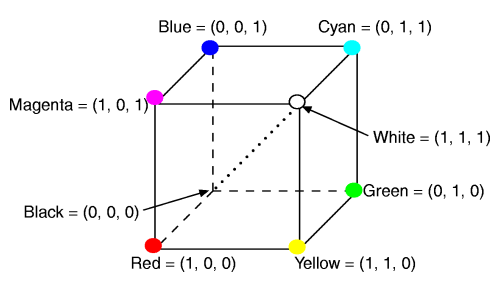
\includegraphics[scale=0.5]{figuras/modelo_rgb}}
    \caption{Representação do modelo RGB através do desenho de um cubo \cite{MOTTA}.}
    \label{img:modelo_rgb}
\end{figure}

\subsubsection{Modelo HSV}

O modelo HSV apresenta uma forma diferente de representar as cores, onde se tem a matiz (\textit{hue}), saturação (\textit{saturation}) e valor (\textit{value}). A matiz é responsável por determinar a tonalidade dominante de uma área, ou seja, a família em que aquela cor está inserida. Esse componente é medido através de valores entre 0 e 360. A saturação mede a pureza da cor da área. Já o valor define a luminância da cor. Nas modalidades de saturação e valor, a variação pode ocorrer entre 0\% e 100\%.

Conforme visto na Figura \ref{img:modelo_hsv}, o espaço de cor HSV é representado por um cone. O lado circular do cone apresenta as tonalidades, normalmente representadas por um ângulo, onde cada ângulo corresponde a uma cor no cone. A saturação é representada pela distância desde a borda ao centro do círculo, de modo que, quanto menor o valor de saturação, menor a presença de tons de cinza na imagem e mais próxima da cor branca. O brilho é determinado pela posição vertical em cores do cone. Na extremidade pontiaguda do cone, não há nenhum brilho, portanto a tonalidade das cores se aproximam da cor preta. No final do cone, na base, estão as cores mais brilhantes \cite{DARRIN}.

\begin{figure}[H]
    \centering
    {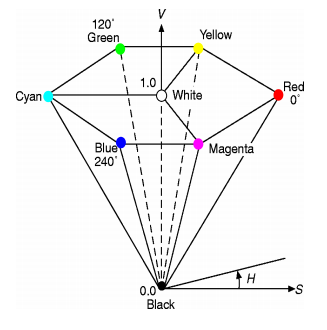
\includegraphics[scale=0.5]{figuras/modelo_hsv}}
    \caption{Representação do modelo HSV através do desenho de um cone \cite{MOTTA}.}
    \label{img:modelo_hsv}
\end{figure}

\subsection{Histograma}

Originalmente criados para melhor análise de dados estatísticos, os histogramas consistem em retângulos contíguos com base nas faixas de valores da variável e com área igual à frequência relativa da faixa. A altura de cada retângulo é denominada densidade de frequência definida pelo quociente da frequência relativa pela amplitude da faixa \cite{CECIRE}.

Em Processamento de Imagem a técnica de histograma é muito utilizada para indicar o percentual de diferentes tons de cinza dos \textit{pixels} em uma imagem através de um gráfico de barras, possibilitando dessa forma uma interpretação visual da distribuição dos valores dos tons de cores da imagem \cite{OGE}. Através da visualização do histograma de uma imagem é possível obter uma indicação de sua qualidade quanto ao nível de contraste e quanto ao seu brilho médio, determinados pela linha horizontal do gráfico. Entretanto, quando uma imagem é colorida, torna-se necessário a decomposição da mesma para que seja avaliado o histograma de cada um dos componentes da imagem separadamente (Figura \ref{img:ex_histograma}).

\begin{figure}[h]
    \centering
    {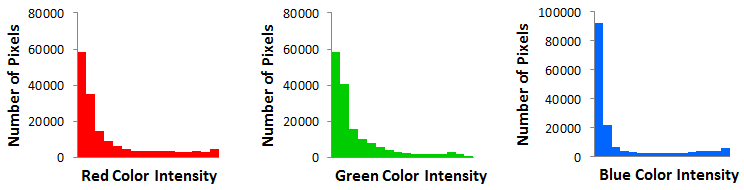
\includegraphics[scale=0.75]{figuras/ex_histograma}}
    \caption{Exemplo de gráficos de histogramas divididos nos canais de cores vermelho, verde e azul \cite{CLOUD}.}
    \label{img:ex_histograma}
\end{figure}

\section{Segmentação}

Além de ser um processo de Visão Computacional, a Segmentação possui uma ligação com a fase de Processamento de Imagem, visto que a qualidade da visualização interfere muito devido à dificuldade de se interpretar as características da imagem. O processo de Segmentação consiste em dividir a imagem em diferentes regiões, buscando separar áreas da imagem, que serão processados posteriormente no processo de Reconhecimento \cite{PUZICHA}.

Nesse processo, existe uma etapa denominada \textit{clustering}, fase de identificação da imagem, que pode ser de dois tipos: supervisionado ou não-supervisionado \cite{ZHOU}. Os processos supervisionados possuem conhecimento prévio sobre quais informações serão classificadas e agrupadas. Em contrapartida, os processos não-supervisionados não requerem nenhuma informação anterior sobre as informações que devem ser agrupadas.

A etapa de Segmentação pode ser realizada utilizando métodos baseados em histograma \cite{ROTHER}, onde são realizados cálculos utilizando um histograma a partir de todos os \textit{pixels} da imagem, e os picos e vales do histograma podem ser utilizados para definir um número d agrupamentos a ser encontrado. Além disso, esse processo também pode ser realizado através de lógica espacial \cite{KOLMOGOROV}, dividindo ou fundindo imagens a partir de pontos semelhantes.

Devido à dificuldade em fazer com que o computador reconheça os padrões e agrupe as imagens significativas, a Segmentação se torna um dos processos mais complexos da área de Visão Computacional. Tomando como base uma imagem que possui diversos objetos distintos, fazer com que o computador interprete e consiga separar esses objetos se tornou um desafio para os técnicos. Consequentemente, surgiram várias técnicas de agrupamentos que buscam no fim o mesmo resultado, ou seja, uma coleção de segmentos que quando combinados formam uma imagem inteira.

Existem várias técnicas e métodos para segmentar uma imagem tanto estática quanto dinâmica. A seguir serão apresentados alguns dos principais métodos de agrupamentos utilizados pelo processo de Segmentação.

\subsection{Segmentação por região}

A detecção por região pode ser feita extraindo uma região ou dividindo a imagem em várias regiões diferentes. As regiões normalmente apresentam como característica a continuidade do nível de cinza de seus pixels e podem ser detectadas pelos métodos de \textit{thresholding} ou dividindo e fundindo segmentos da imagem.

\subsubsection{\textit{Thresholding}}

Várias técnicas podem ser utilizadas para alcançar a seleção de segmentos que formam os objetos buscados pelo sistema. \textit{Thresholding}, também conhecido como limiarização, é o método de Segmentação de fácil compreensão, se comparado com as demais. O método consiste em utilizar imagens pós-processadas e convertidas para tonalidades de cinza em sequência, criando um limiar onde é separada da imagem principal uma imagem segmentada.

O \textit{thresholding} é um método baseado em histograma, onde o limiar de separação pode ser encontrado nos vales entre um pico e outro do histograma \cite{PADILHA}.

\subsubsection{Dividir e fundir}

Como mencionado no método de \textit{thresholding}, a maneira mais simples possível para segmentar uma imagem é selecionando um limiar e então calcular os componentes ligados. Entretanto, um único limiar raramente é o suficiente para a imagem por causa da iluminação e variações estatísticas do objeto \cite{SZELISKI}. O método de dividir e fundir agrupa em segmentos os \textit{pixels} que se encontram em regiões de características semelhantes, dividindo ou fundindo a imagem se preciso.

\subsection{Segmentação por contornos}

O contorno pode ser definido pela variação dos níveis de cinza entre duas regiões semelhantes. O método de detecção de contornos da imagem permite encontrar regiões com uniformidades de valores. Nesse método de Segmentação é localizado a região da imagem que possui variações nos valores. O objetivo do método é localizar as bordas ou curvas dos objetos nas imagens em forma de contornos finos e sem interrupções \cite{SZELISKI}.

Também é possível segmentar uma imagem por contornos através da detecção de pontos. Esse método é muito utilizado em objetos em movimento, avaliando a variação em suas direções principais \cite{ANTUNES}.

\subsection{Segmentação por textura}

A detecção por textura busca agrupar subconjuntos que possuam aproximadamente as mesmas características em qualquer lugar da imagem \cite{ANTUNES}. Essa técnica possui métodos como o estatístico, baseando-se na distribuição dos níveis de cinza da imagem para definir uma matriz que representa essa distribuição através da imagem, e então, a partir dessa matriz, identificar a probabilidade de um conjunto de \textit{pixels} compor uma determinada textura.

\section{Reconhecimento}

Realizar a análise e reconhecimento de objetos em uma cena tem sido uma das tarefas mais desafiadoras no domínio da Visão Computacional. Apesar de ser uma tarefa facilmente executada por crianças, conseguir que um computador realize a mesma tarefa não é igualmente simples \cite{SZELISKI}. A dificuldade no Reconhecimento se dá pela infinidade de classificações que os seres humanos empregam. Ainda é possível acontecer de objetos da mesma classe conterem atributos distintos, dificultando ainda mais a exatidão na fase de Reconhecimento e tornando improvável a análise através de uma base de dados de exemplos.

O objetivo da etapa de Reconhecimento é fazer com que o sistema classifique as informações adquiridas das etapas anteriores baseada em um conhecimento proposto ou com experiência em aprendizado.

Em muitos casos, o Reconhecimento depende do contexto onde o objeto está inserido e os elementos da cena. Se o objeto procurado for de conhecimento do computador, é possível procurar por pontos característicos e verificar se os mesmos se alinham de forma geométrica. Existem vários modelos utilizados para realizar um reconhecimento em uma imagem. Em seus estudos, \citeonline{WEBER} apresenta diversos modelos de Reconhecimento balanceados por funções probabilísticas.

Um dos modelos mais simples apresentados é caracterizado por um objeto constituído pela formação de várias peças que podem possuir características distintas, como aparência, forma e escala relativa. A partir da segmentação das peças do objeto é iniciada a fase de detecção, que em uma primeira etapa utiliza detectores especializados para cada uma das peças formadas. Após as peças serem reconhecidas e suas informações armazenadas, a segunda etapa é iniciada para a detecção do objeto formado através da união das informações de cada peça recolhida. Outra etapa importante no processo é a localização do objeto na imagem, que é realizada usando as peças detectadas que correspondem ao objeto em primeiro plano na imagem.

Através desse modelo, conseguiu-se um reconhecimento razoavelmente rápido e simples. Além disso, a partir desse modelo, Weber propôs outros modelos que utilizavam cálculos com funções buscando um custo de processamento menor.
